\section{Experiments}
\label{sec:exp}

\subsection{Datasets}
Our experiments aim to study the short text classification in the low-resource
environment  popular  in  the  task-specific conversational chatbot application.
Hence we choose and configure datasets to serve this study. Different from
the  datasets from other short text classification research, such as semantics
classification  with  very  limited  semantics labels and relatively longer
input,   the   datasets  adopted  in  our  experiments   typically  contain
comparatively  large  number  of  class labels, ranging from several dozens to
hundreds,  and  each  class  label  is  associated  with  a handful of labeled
queries with each  query  being usually  one  sentence. Table \ref{tbe:dataset
statistic} displays their statistics.  All settings of six public datasets would 
be released to github soon.

\begin{enumerate}
  \item \emph{ITG},  is  a proprietary FAQ dataset from real-world
  chatbot  project,  which is composed of question and answer pairs about online
  English teaching. It contains 3,938 sample questions for 228 class labels, and
  each class label corresponds to a unique answer.

  \item \emph{Amazon-670K}, is a customer product review dataset for
  text  classification  task  from  the  extreme  classification repository. The
  complete  dataset  contains 670,091 class labels, 285,176 training samples and
  150,875   testing   samples   \cite{bhatia2016extreme}.  As  each  sample  may
  correspond  to  multiple  class labels, we keep only the first one. We further
  filter  out the class labels that only associated to training samples within the amount of 5 to 15 to  mimic  the  few-shot chatbot scenario. From them, we sample 250 class
  labels as well as their training samples to form a subset with 2658 samples.

  \item \emph{HWU64}, is an intention detection dataset designed for
  home  robot  scenario \cite{liu2019benchmarking}. It aims at the specific task
  of  capturing  the  intention  for  different  user requests to home robot and
  finding  the corresponding answer. The raw dataset contains 25,716 data points
  for 64 class labels through crowdsourcing.

  \item \emph{CLINC150},  is  a dataset designed for task-oriented
  systems  with  23,700 queries that are short and unstructured for 150 intents,
  in    the    same   style   made   by   real   users   through   crowdsourcing
  \cite{larson2019evaluation}.

  \item \emph{BANKING77}, is an intention detection dataset for bank
  customer  services.  The  raw dataset contains 13,084 data points for 77 class
  labels \cite{casanueva2020efficient}.
  
  \item \emph{FRAMES}, is a collection of multi-domain dialogues dealing with
hotel bookings. The raw data is consists of 1369 human-human
dialogues with slot filling information. There are 30,522 utterances in total for 21 intents and 49 slots \cite{asri2017frames}.

  \item \emph{ATIS}, is a popular dataset for intent detection of flight reservations with slot filling\cite{tur2010left}. The raw data's training, development and test sets contain 4,478, 500 and 893 utterances, respectively. There are 120 slot labels and 21 intent types for the training set.

\end{enumerate}

Regarding  the first two datasets, we conduct 3-fold cross validation experiments
that   70   percent   as  training,  15  percent  as  validation  and  testing
respectively,  and  report  the  averaged  testing results. Regarding the last
five datasets, we conduct experiments using a sampling method similar to that
in   \cite{casanueva2020efficient}   yet  in  a  more  sophisticated  few-shot
settings.  We  fix  a  test  data for each one, and examine their performances
using  5,  10,  15,  20,  30,  or 50 samples per class label respectively for
training.  This  is important, as in practice, a task-specific chatbot usually
starts  with  merely  a  handful of labeled data available in the early stage.
Besides,  in  the  active  learning framework, building an effective auxiliary
system  with limited resource is also quite important to help developers label
data more efficiently.

\subsection{Baselines}
We  choose  four kinds of system as our baselines. All our pretrained
model   baselines  are  fine-tuned  on  our datasets.
Especially, the similarity  model  baseline  and all similarity modules in SFCs
use extra Quora  dataset  \cite{iyer2017first}  to enhance system performance.

\begin{enumerate}
  \item \emph{Pretrained model based classification system}, which consists of
  BERT \cite{devlin2018bert},  RoBERTa \cite{liu2019roberta},  and  ALBERT  \cite{lan2019albert}  based.  These pretrained
  models  are  practically  proven  to  achieve  outstanding  performances  in
  classification task and other NLP tasks.

  \item   \emph{Non-pretrained   model  based  classification  system},  which
  consists  of  a typical CNN based TextCNN \cite{kim2014convolutional}, and a
  label-embedding based LEAM \cite{wang2018joint}. Regarding TextCNN, the
  model is based on output from RoBERTa tokenization, and the kernels are set
  as 1, 2, 3, 4, 5. Regarding LEAM, a literal class label is required, which
  is available only in HWU64, CLINC150, BANKING77. Thus, for other two
  datasets, we have to use its class number instead.  Empirically,
  a  non-pretrained  model  based  system  are  not  performing  as  well as a
  pretrained  models  based,  if  both is applicable in some task. Our listing
  these  non-pretrained model based systems here is to provide a comprehensive
  performance comparison on our datasets.

  \item   \emph{Pre-trained   model   based   similarity   model}.  We  choose
  RoBERTa-large  as  our  fundamental  module as our SFC systems are based on
  RoBERTa  too, and RoBERTa is empirically more effective than other pretrained
  models  in  the  short  text  classification  task  in  our  experiments. In
  inference,  we  use  an  elastic search to find a set of potential candidate
  labels for the similarity model, to guarantee a reasonable running time.
  
  \item \emph{Pre-trained model based text classification and NER joint model}. Considering  a  joint  model,  our  SFC framework  is also supportive of NER task. That  is  in  stage  1,  based on the  output  states from a
pretrained model, we can derive a fourth task for NER loss. For performance comparison, we choose the state-of-the-art model, which is RoBERTa-large with NER loss, using the same model structure with \cite{chen2019bert}, as our baseline.
\end{enumerate}

Our SFC systems include two-stage SFC with ablation, trained with two tasks
separately and both, and joint SFC with all three tasks. All setting details can
be found in the appendix due to the space limitation.

\subsection{Result Analysis}
We  report  the F1 score \footnote{In the multi-class and multi-label case, this
is  the  average  of  the F1 score of each class with weighting depending on the
numbers  in  each class.} as the main evaluation measure for all experiments in
Table \ref{tbe:table2} and Table \ref{tbe:addtional ner experiments}.

\subsubsection*{Are multi-task and joint training working?} 
First, we compare the four  SFC  variants shown in Table \ref{tbe:table2} to analyze the improvement
brought  by  multi-task  and  joint-model  structure. 

\begin{table}
  \begin{centering}
    \scalebox{0.58}{
      \begin{tabular}{|c|ccc|ccc|}
        \hline
        \multicolumn{1}{|c|}{\multirow{2}*{\textbf{Models}} }& \multicolumn{3}{c|}{\textbf{FRAMES}}& \multicolumn{3}{c|}{\textbf{ATIS}}\tabularnewline
        \cline{2-7}
        \multicolumn{1}{|c|}{} & $\textbf{10}$ & $\textbf{20}$ & $\textbf{50}$
        & $\textbf{10}$ & $\textbf{20}$ & $\textbf{50}$\tabularnewline
        \hline
        RoBERTa-large & \multirow{2}*{${0.3456}$} &
        \multirow{2}*{${0.4043}$} & \multirow{2}*{${0.4262}$} &
        \multirow{2}*{${0.9349}$} & \multirow{2}*{${0.9757}$} & 
        \multirow{2}*{${0.9800}$}\tabularnewline
        (classification) & & & & & & \tabularnewline
        \hline
        RoBERTa-large & \multirow{2}*{${0.3520}$} &
        \multirow{2}*{${0.4088}$} & \multirow{2}*{${0.4353}$} &
        \multirow{2}*{${0.9560}$} & \multirow{2}*{${0.9706}$} & 
        \multirow{2}*{$\textbf{0.9832}$}\tabularnewline
        (classification w/ NER) & & & & & & \tabularnewline
        \hline
        Joint SFC & \multirow{2}*{${0.3843}$} &
        \multirow{2}*{${0.4130}$} & \multirow{2}*{${0.4390}$} &
        \multirow{2}*{${0.9618}$} & \multirow{2}*{${0.9761}$} & 
        \multirow{2}*{${0.9825}$}\tabularnewline
        (w/o NER) & & & & & & \tabularnewline
        \hline
        Joint SFC & \multirow{2}*{$\textbf{0.3925}$} &
        \multirow{2}*{$\textbf{0.4420}$} & \multirow{2}*{$\textbf{0.4456}$} &
        \multirow{2}*{$\textbf{0.9639}$} & \multirow{2}*{$\textbf{0.9784}$} & 
        \multirow{2}*{${0.9826}$}\tabularnewline
        (w/ NER) & & & & & & \tabularnewline
        \hline
      \end{tabular}
    }
      
  \end{centering}
  \caption{F1 scores on two task-specific datasets for joint training of sentence classification and NER in chatbot domain under low resource. For both FRAMES and ATIS, we set up various few-shot settings(10/20/50 samples per intent) while keeping the original test set.}
  \label{tbe:addtional ner experiments}
\end{table}

\begin{table}
  \begin{centering}
    \scalebox{0.85}{
        \begin{tabular}{|c|c|c|c|}
        \hline
        F1 score & Two-stage SFC & Joint SFC & Gap \tabularnewline
        \hline
        top-1 accuracy  & \textbf{81.50} & 81.07 & -0.47 \tabularnewline
        top-5 accuracy & 94.01 & \textbf{94.30} & +0.29 \tabularnewline
        \hline
      \end{tabular}
    }
    \par
  \end{centering}
  \caption{The average classification accuracy in percentage in stage 1 on all five dataset.}
  \label{tbe:top1_5_accuracy}
\end{table}

Comparing with training two-stage SFC with multi-task, training with only task
1,  namely the sentence pair similarity model, degrades by 0.8 percent
point  on average, and training with only task 2, namely the top-K based
classification  task,  degrades  by  0.45  percent  point  on  average.  These
degradation  indicates  multi-task training in two-stage SFC is helpful for the
system  performance.  Besides, task 2 plays a relatively more important role in
multi-task learning, and this aligns with their optimal weight settings.

Joint SFC consistently outperforms two-stage SFC with multi-task training  
on 5 diverse datasets by 0.95 percents  on  average. 
This observation supports the idea that the joint model
structure  can  alleviate  the  limitation  brought by the lack of interaction
between  two  stages.  In  following analysis, we will focus on the comparison
between joint SFC and the other baseline models.

\subsubsection*{Is  the  fusion of classification and similarity models
helpful?}  We  compare  joint SFC with classification, similarity and NER joint model based baselines respectively.

\begin{table*}
  \begin{centering}

    \begin{tabular}{|c|c|c|c|c|c|c|}
      \hline 
      \multicolumn{1}{|c|}{\multirow{2}*{Dataset}}&\multicolumn{1}{c|}{\multirow{2}*{Model}}& $K=3$ & $K=5$ & $K=10$ & $K=15$ & $K=20$\tabularnewline
      \multicolumn{1}{|c|}{} & \multicolumn{1}{c|}{} & $P=20$ & $P=10$ & $P=5$ & $P=4$ & $P=3$\tabularnewline
      \hline
      \multicolumn{1}{|c|}{\multirow{2}*{ITG}}& two-stage SFC & $0.8034$ & $0.8124$ & $0.8008$ & $0.7967$ & $0.7934$\tabularnewline
      \cline{2-7}
      \multicolumn{1}{|c|}{} & joint SFC & $0.7986$ & $0.8114$ & $0.8010$ & $0.7972$ & $0.7918$\tabularnewline
      \hline
      \multicolumn{1}{|c|}{\multirow{2}*{Amazon-670k}}& two-stage SFC & $0.7278$ & $0.7364$ & $0.7366$ & $0.7328$ & $0.7204$\tabularnewline
      \cline{2-7}
      \multicolumn{1}{|c|}{} & joint SFC & $0.7334$ & $0.7445$ & $0.7516$ & $0.7344$ & $0.7373$\tabularnewline
      \hline
    \end{tabular}
    \par
  \end{centering}
  \caption{
    We  show the performances of SFC from different settings of
    hyperparameters, $K$  denoting the candidate class number from stage 1,
    $P$ denoting the number of sampled sentence pair in stage 2. 
  }
  \label{tbe:table3}
\end{table*}

Regarding the  classification  models,  joint SFC
outperforms RoBERTa-large based, the strongest among all baselines, 
by 2.04 percent points on average F1 score over 5 datasets.  
Especially, ALBERT.xxlarge based is rather unstable  in this scenario. Thus, 
we did multiple run with different settings and  report the  best  ones here. 
Comparatively,  RoBERTa  based is  the  most stable and has the best performance 
n almost all experiment settings.

Regarding  the  similarity  model,  as  analyzed  above,  we  only  choose the
RoBERTa-large based implementation as our baseline. Joint SFC achieves more improvement of
7.09  percent points  on average F1 score. 

As for the intent classification and NER joint model, we choose the state-of-the-art RoBERTa-large model with NER loss as our strongest baseline. For ablation study, we did experiments on Joint SFC model with and without NER loss respectively. From Table \ref{tbe:addtional ner experiments}, we can see that our Joint SFC without NER loss still outperforms RoBERTa with NER loss baseline by 0.86 percent points on average. This indicates that the fusion of classification and similarity can even works better than fusing with additional NER information under few-shot chatbot scenario. Moreover, after adding NER loss to Joint SFC, it achieves further improvement by 1.66 percent points over RoBERTa with NER loss baseline. Especially for FRAMES dataset, which is a much more difficult task in comparison with ATIS, our Joint SFC with NER loss achieves a bigger improvement of 2.8 percent points on average. In this way, we show the compatibility of our Joint SFC model with extra semantic information, as well as the stable outstanding performance of Joint SFC when facing hard tasks with few training data.

The above analysis illustrates that suitable fusing these two kinds of models
can take their advantages.

\subsubsection*{Does joint SFC improve the classification in stage 1?}
We  compare  the  top-1  prediction and top-5 candidate labels in stage 1 from
two-stage SFC and joint SFC in Table \ref{tbe:top1_5_accuracy}. We should note
that  two-stage  SFC  does not optimize the stage 1 model, which is a RoBERTa
based classification model.

The joint training does not improve the classification performance in stage 1,
measured  by  top-1  accuracy.  However,  it  improves  the  quality of top-5
candidate  class  labels, which can further improve the effect of sentence pair
similarity training. The reason is that, a classification model
inherently optimizes the objective loss, 0-1 error of top-1 here; the sentence
pair similarity model in the joint SFC poses more positive effect in optimizing the 
candidate labels.


\subsubsection*{How does training sample size influence SFC?} 
We analyze the overall  improvement  trend  of  joint SFC under various few-shot
settings, and show results in Fig. \ref{fig:trend}.

Our main focus  is  to  study  chatbot  building  in common situation during real-world
application  where  only  a few sample sentences are available for each class.
The  experimental  results  for  the  3  diverse  intention detection datasets
(ClINC150,  BANKING77,  HWU64)  under  few-shot  settings, 5 to 50 samples per
class,  indicate that our proposed joint SFC can achieve 2.47 percents average
improvement   over  one  of  the  most  powerful  baseline  models,  which  is
RoBERTa-large  classification  model.  Moreover,  the  improvement  in F1 score
becomes  more  and  more prominent with the decrease of data sample number per
class.

\begin{figure}[t]
  \begin{centering}
    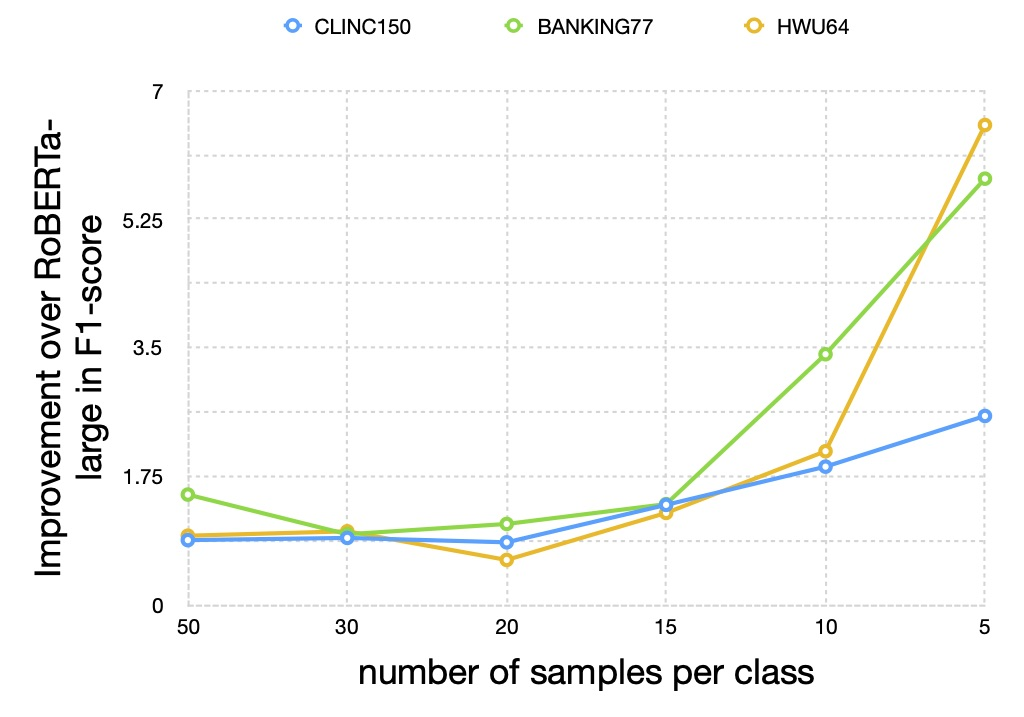
\includegraphics[scale=0.2]{picture/improvement_trend.jpg} 
    \par
  \end{centering}
  \caption{
    Improvements  from  Joint  SFC  over  RoBERTa  based  classification  with
    different size of training data.
  }
  \label{fig:trend}
\end{figure}

Especially,  in the most extreme few-shot setting with only 5 training samples
per  class  our joint SFC achieves 4.97 percent points improvements on average
over  RoBERTa-large classification model. This observation indicates that SFC
is  especially  well-performed  when being applied during the initial stage of
building  task-specific  chatbot  system,  where the amount of data sample for
each class label is extremely scarce.

Furthermore,  our  proposed  joint  SFC can also achieve 2.04 percents average
improvement  over  RoBERTa-large classification model on all the data settings
including  the  ones  with  large  scale,  30  to  50  samples per class. This
indicates that joint SFC can still steadily outperforms pretrained model based
baseline even if the data size grows bigger. However, the improvement is still
more prominent when the data is scarce, which makes SFC an excellent model for
low-resource chatbot scenario.

\subsubsection*{How does joint SFC relate to the label  embedding based  LEAM?}
LEAM performs consistently better than TextCNN by a large margin in all
datasets. TextCNN is practically efficiently in task-specific chat
applications, and LEAM shows its power in modeling labeling information.

LEAM  does not perform as well as SFCs, since the first intuitive reason is it
does  not use pretrained model as encoding module; and another critical reason
is  in  task-specific  chat applications, it is common to have many intentions
that are close to some others with a minor difference, and it is hard and even
impossible  to  name  each  intention  with  a short clear name. One candidate
solution  is  setting  a most standard sample as the label of that class. When
using  non-pretrained  models  base  LEAM,  this is applicable. Yet when using
pretrained  model  based, as the all labels can be hundreds of thousands, then
this  can not be accommodated in a poplar 32 G Tesla V100 GPU. Actually, joint
SFC  can  be  kind  of  understood  as  a  generalization form of LEAM. In the
scenario when there is no clear class label, the relationship between a sample
and  a class label is implicitly encoded as that between a sample and another
sample  from  the  same  class, and this turns into a sentence pair similarity
model.


